\section{Real time anomaly detection with Kinesis - Clemens}
\label{sec:real_time_anomaly_detection}
    \subsection{Motivation}
    This approach is inspired by a Medium blog post\cite{MEDIUM}. 
    \footnote{\scriptsize{\url{https://medium.com/@devfire/real-time-anomaly-detection-in-vpc-flow-logs-part-1-introduction-55ed000e039b}}}
    The goal of the approach is to move the anomaly detection closer to a real-time setup. This means to continuously process the most recent data instead of analyzing data from the previous month or year to find anomalies. To give some more motivation about why this is actually an important issue, here is a quote from a job description from Netflix\cite{NETFLIX}:
    \begin{displayquote}
        "Netflix Operational Insight Team is the team responsible for building common infrastructure to collect, transport, aggregate, process and visualize operational metrics. We build powerful systems to allow everyone at Netflix visibility into the state of our environment at both a macro and micro level."
    \end{displayquote}
    The fact that a leading and modern company like Netflix builds a whole team just dedicated to checking and visualizing the current system state in real time, underlines how important it is to know at every moment how your environment performs.\\
    AWS Kinesis is a very suitable tool for this problem for multiple reasons. First of all, Kinesis is designed to process streaming data. This means we can ingest real-time data which is a perfect fit for our given VPC flowlog data. Second Kinesis comes with Kinesis Data Analytics already built in. Amazon Kinesis Data Analytics offers easy ways to analyze streaming data, gain actionable insights, and respond to business needs in real time. In addition to that there is a SQL function called “Random cut forest with explanation” which is described by AWS as follows:
    \begin{displayquote}
        Computes an anomaly score and explains it for each record in your data stream. The anomaly score for a record indicates how different it is from the trends that have recently been observed for your stream. The function also returns an attribution score for each column in a record, based on how anomalous the data in that column is. For each record, the sum of the attribution scores of all columns is equal to the anomaly score. \cite{awsRcf}
    \end{displayquote}

    \subsection{Architecture}
    So with this prior knowledge let’s jump right into the system setup.
    First let’s get an overview of the system as it was implemented during the project phase:
    \begin{figure}
        \centering
        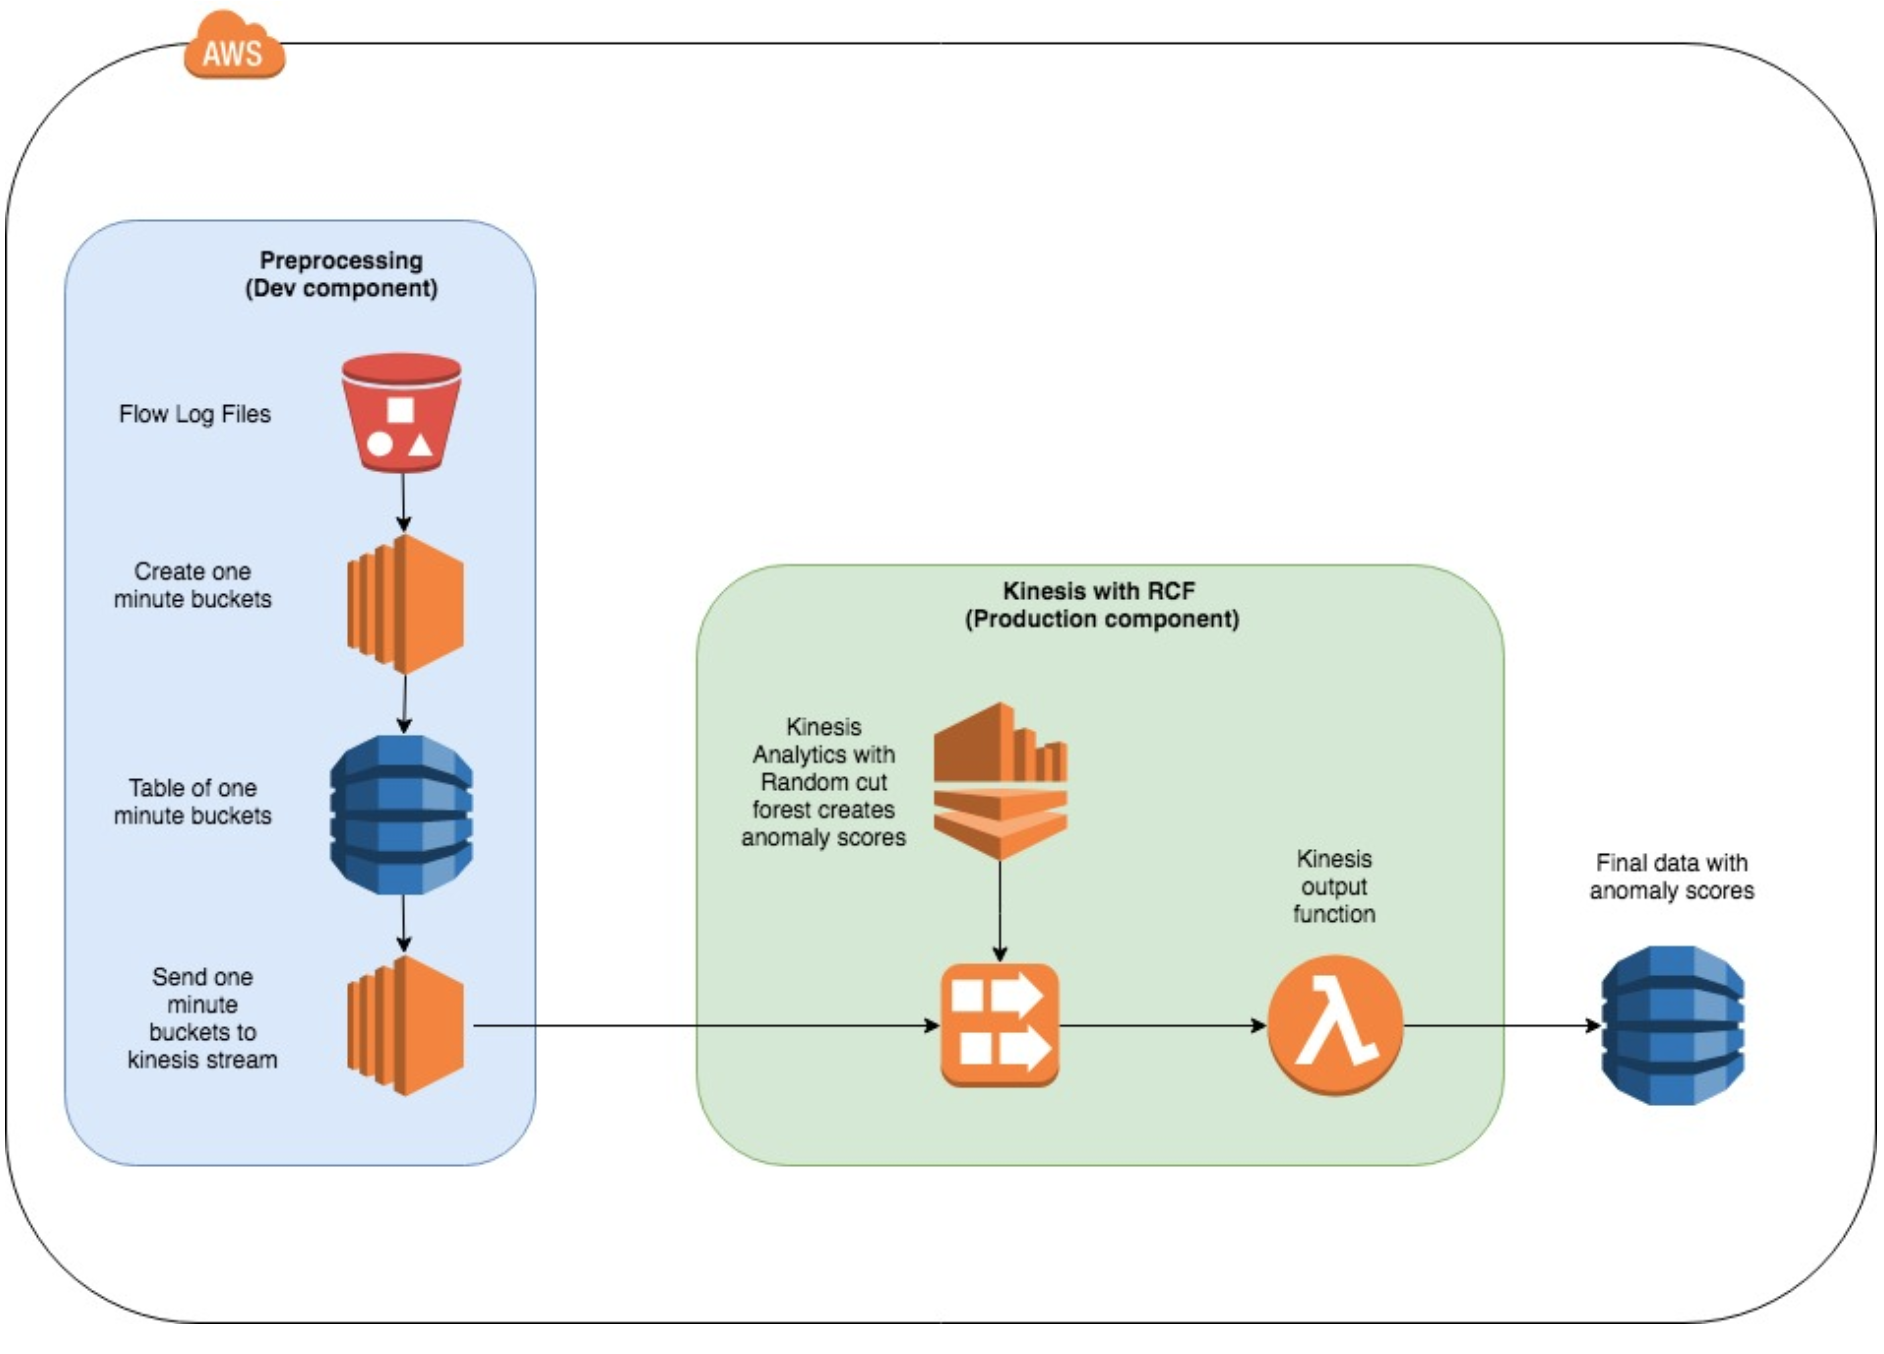
\includegraphics[width=1\textwidth]{images/medium-kinesis-setup.png}
        \caption{Medium Kinesis Random Cut Forest Setup}
        \label{fig:medium_kinesis_setup}
    \end{figure}
    \FloatBarrier
    First of all it should be noted that all the preprocessing components on the left (blue area in figure \ref{fig:medium_kinesis_setup}) would not be part of a production system. In a production system we would have a continuous stream of VPC flow logs which needs to be handled and preprocessed, whereas in the project setup we had all the flow logs data from the past in a S3 bucket. 
    
    \subsection{Preprocessing components (blue area in figure \ref{fig:medium_kinesis_setup})}
    In the following section we will look at the preprocessing setup in detail, keeping in mind that this is not created to run in production.
    
    \paragraph{S3: Flow Log Files}
    All the flow logs data provided by BMW lies in an S3 bucket called \textit{fog-bigdata-bmw-data}. As mentioned in \pageref{sec:fixed_data}, there are two types of data: first the metrics, which already contain summaries about how many requests were made to the system during a certain time interval. Another issue here was, that the time intervals are of different size (sometimes five minutes, sometimes four or six or something similar). Of course this is not a good basis to run our anomaly detection, because we cannot know what value we expect (since the size of the intervals are different). Therefore the second type of data is more suitable, namely the raw VPC Flowlogs. However, we want to look at how many requests are made to our system per minute and therefore we need to do some preprocessing.
    
    \paragraph{EC2: create one minute buckets}
    This is where the first script with the name \textit{createOneMinuteBuckets.py} comes in. This script is executed on an EC2 instance and reads all the flow log records from the S3 bucket. It creates one-minute buckets from the Flowlogs, so that we know for every one minute time interval how many requests were made to the system. 
    
    \paragraph{DynamoDB: table of one minute buckets}
    The information about these one minute buckets is then written into a DynamoDB table (called \verb|medium_bmw_data_to_kinesis|). For the sake of this project the data from the Kinesis table was then exported to a CSV file and the information about the weekdays was added (currently done in Excel). This means that for every one minute bucket we know the hour and the minute and also on which weekday it was recorded. This might be relevant because the expected number of request at 8am on a Sunday can be very different than 8am on a Monday, especially because the requests come from driving cars.  Of course this step will not be part of a production system (as mentioned before).
    
    \paragraph{EC2: send one minute buckets to Kinesis stream}
    The next script is called \textit{generateAnomalyScores.py}. The script and the final CSV file is uploaded to EC2 again. The script takes the data from this CSV file and sends it to the kinesis Stream called medium\textunderscore VPCFlowLogs. An alternative setup could be to read the data directly from DynamoDB and add the information about the weekday in the python script (instead of using CSV and Excel).\\
    This is where the preprocessing part (which would look different in a production system) ends and where the production component (green area in figure \ref{fig:medium_kinesis_setup}) comes into play.\\
    
    \subsection{Production component (green area in figure \ref{fig:medium_kinesis_setup})}
    In this section we assume that we already have all the data we need in the right format. This is the part of the system where the actual anomaly detection happens. This part of the the setup can be used in a production environment in the same or in a similar way. All the preprocessing is done and the data is already fed into the our Kinesis stream.
    \begin{figure}
        \centering
        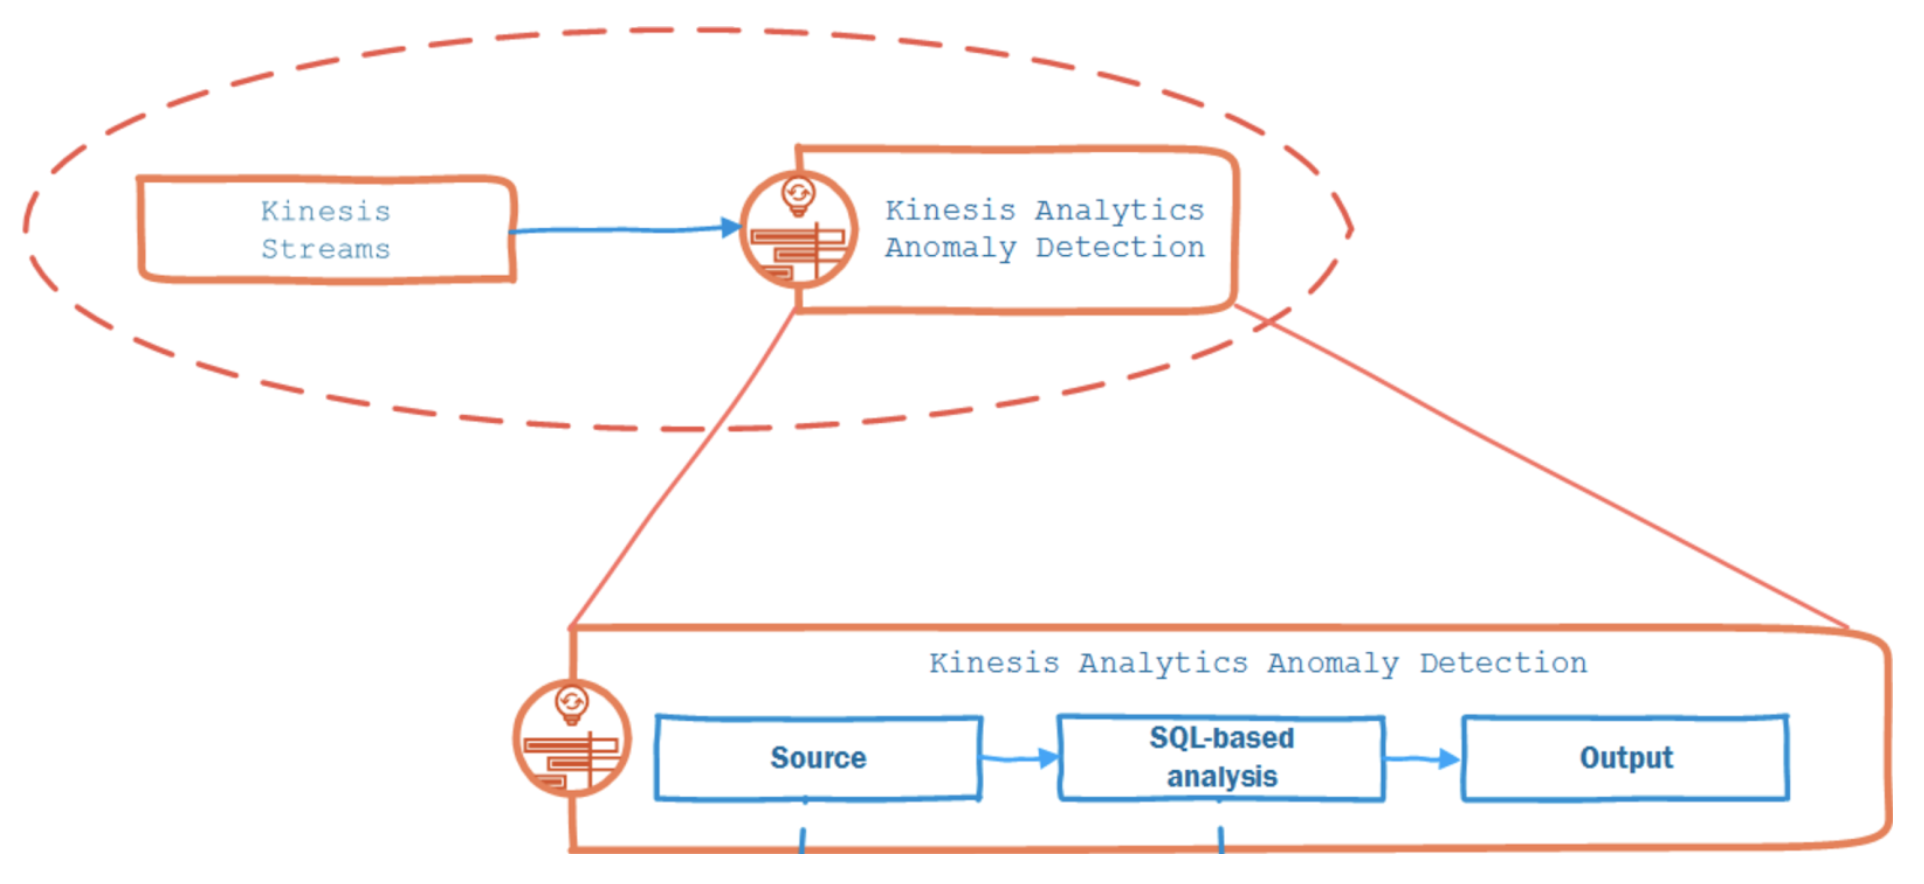
\includegraphics[width=1\textwidth]{images/kinesis-rcf.png}
        \captionsource{Kinesis Data Analytics with RCF}{\scriptsize{Source: https://medium.com/@devfire/real-time-anomaly-detection-in-vpc-flow-logs-part-5-anomaly-detection-d1fc9b61baf8}}
        \label{fig:medium_kinesis_data_analytics_rcf}
    \end{figure}
    \FloatBarrier
    The Kinesis stream has a Kinesis Data Analytics application which sends the data to random cut forest where the anomaly scores are created. This is the SQL code for the real time analytics:
    \begin{figure}
        \centering
        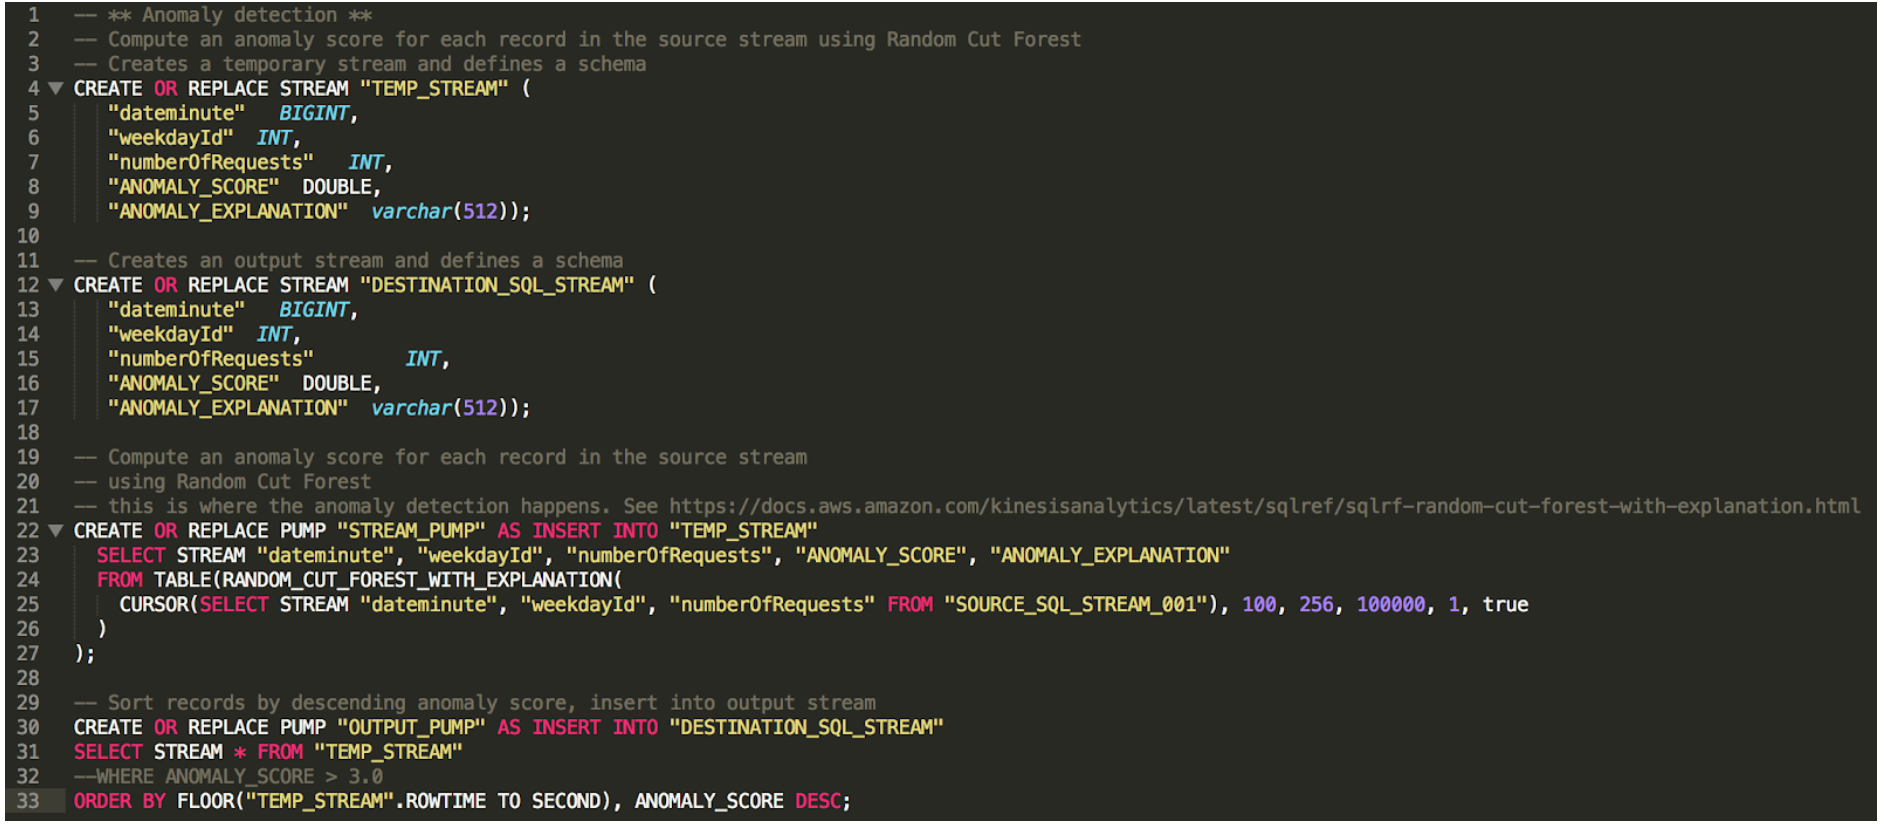
\includegraphics[width=1\textwidth]{images/sql-analytics.png}
        \captionsource{SQL code for real time analytics}{\\\scriptsize{Source: https://medium.com/@devfire/real-time-anomaly-detection-in-vpc-flow-logs-part-5-anomaly-detection-d1fc9b61baf8}}
        \label{fig:medium_sql_analytics}
    \end{figure}
    \FloatBarrier
    As we can see from the comment in line 32 it would be possible to already define a threshold here. This would then mean, that only anomaly scores which are higher than that specified threshold are sent to the output stream. However it is recommended to do implement this threshold in the output lambda function, to keep the threshold logic separate from the creation of the anomaly scores. Furthermore it is a lot easier to version and backup the lambda function in case the threshold is changed over time than to maintain different versions of the SQL code in the Kinesis Data Analytics part.
    \paragraph{Lambda: Kinesis output function}
    The output of the kinesis stream is sent to the Lambda function \verb|medium_bmw_kinesis_to_dynamodb_2|. \\
    This Lambda function just stores the results to another DynamoDB called \verb|kinesis_bmw_anomaly_scores|. Obviously this last database table was just for the purpose of the project phase to collect all the anomaly scores and visualize them in a graph but it is not needed in a production setup (as indicated in the system architecture). Instead in a production system this output function should contain the threshold for the anomaly score and then send a message or trigger a phone call if the threshold is exceeded.
    
    \subsection{Results}
    \begin{figure}[h]
        \centering
        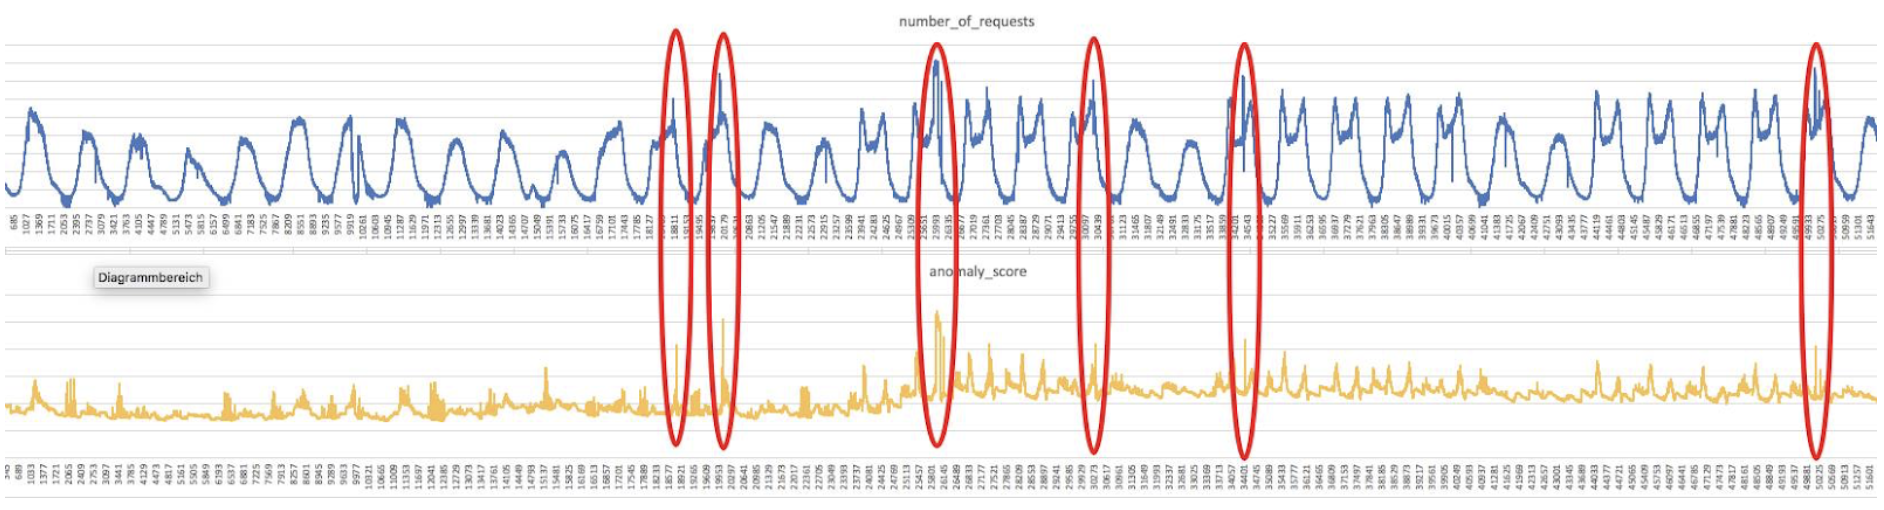
\includegraphics[width=1\textwidth]{images/kinesis-results.png}
        \caption{Visualisation of Kinesis Analytics Results}
        \label{fig:medium_kinesis_results}
    \end{figure}
    \FloatBarrier
    The blue graph at the top of figure \ref{fig:medium_kinesis_results} shows the requests to the the system per minute (from the one minute buckets). The orange graph at the bottom of figure \ref{fig:medium_kinesis_results} visualizes the anomaly score at that time. This means if we see an unexpected high peak or unexpected low drop in the first graph (number of requests per minute), in both cases we would expect a peak in the second graph (the anomaly scores). All in all this example does not show a perfect result (since we would expect our anomaly scores to be consistently low when there is no anomaly), however we have to take into account that this particular data set show the requests from December 21, 2018 until January 28, 2019 which means that it starts with the Christmas holidays which does not show the normal pattern of five weekdays followed by two weekends which we see towards the end.\\ Furthermore this is a series of 54,689 one minute buckets which is not a very long series to train on. Despite these factors of having limited and atypical data the high spikes in the anomaly scores (highlighted by the red ellipses) indicate that the approach in general is quite promising and that it can already detect anomalies.
    
    \subsection{Future work}
    The presented results are retrieved from feeding the data into the random cut forest in the following format: date-minute data, the weekday ID (as an integer) and number of requests.
    To refine the system further it might be interesting to try different combinations of these three input variables to see which combination gives the best results. This way it could be determined if it decreases the performance if we leave out the information about the weekday completely for example.
    
    \subsection{Implementation guide (Kinesis Random Cut Forest)} 
    This can be found in the appendix of this report (Appendix \ref{appendix-medium}) or online at \url{https://gist.github.com/clemenspeters/8e9025e3bd71e9087df154fb06f96328}